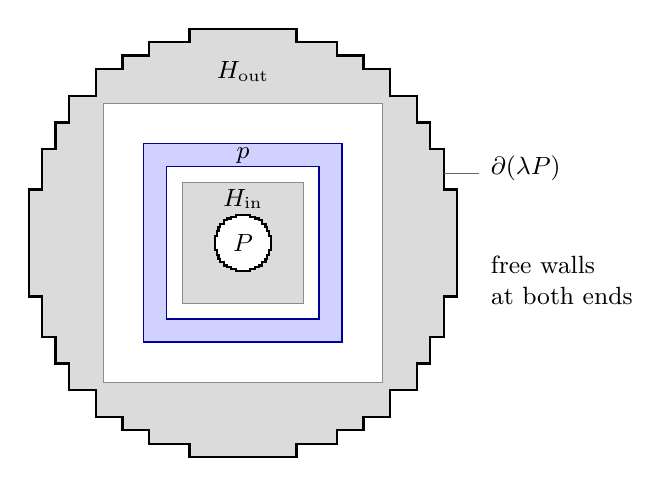
\begin{tikzpicture}[scale=.68, every node/.style={font=\small}]
 \def\wall{(4,0)--(4,1)--(3.75,1)--(3.75,1.75)
 --(3.5,1.75)--(3.5,2.25)--(3.25,2.25)--(3.25,2.75)
 --(2.75,2.75)--(2.75,3.25)--(2.25,3.25)--(2.25,3.5)
 --(1.75,3.5)--(1.75,3.75)--(1,3.75)--(1,4)
 --(-1,4)--(-1,3.75)--(-1.75,3.75)--(-1.75,3.5)
 --(-2.25,3.5)--(-2.25,3.25)--(-2.75,3.25)--(-2.75,2.75)
 --(-3.25,2.75)--(-3.25,2.25)--(-3.5,2.25)--(-3.5,1.75)
 --(-3.75,1.75)--(-3.75,1)--(-4,1)--(-4,-1)
 --(-3.75,-1)--(-3.75,-1.75)--(-3.5,-1.75)--(-3.5,-2.25)
 --(-3.25,-2.25)--(-3.25,-2.75)--(-2.75,-2.75)--(-2.75,-3.25)
 --(-2.25,-3.25)--(-2.25,-3.5)--(-1.75,-3.5)--(-1.75,-3.75)
 --(-1,-3.75)--(-1,-4)--(1,-4)--(1,-3.75)
 --(1.75,-3.75)--(1.75,-3.5)--(2.25,-3.5)--(2.25,-3.25)
 --(2.75,-3.25)--(2.75,-2.75)--(3.25,-2.75)--(3.25,-2.25)
 --(3.5,-2.25)--(3.5,-1.75)--(3.75,-1.75)--(3.75,-1)
 --(4,-1)--cycle}
 \fill[black!14] \wall;
 \fill[white] (-2.6,-2.6) rectangle (2.6,2.6);
 \fill[blue!18] (-1.85,-1.85) rectangle (1.85,1.85);
 \fill[white] (-1.42,-1.42) rectangle (1.42,1.42);
 \fill[black!14] (-1.125,-1.125) rectangle (1.125,1.125);
 \draw[black!45] (-2.6,-2.6) rectangle (2.6,2.6);
 \draw[blue!60!black] (-1.85,-1.85) rectangle (1.85,1.85);
 \draw[blue!60!black] (-1.42,-1.42) rectangle (1.42,1.42);
 \draw[black!45] (-1.125,-1.125) rectangle (1.125,1.125);
 \draw[thick] \wall;
 \begin{scope}[scale=.13]
  \fill[white] \wall;
  \draw[thick] \wall;
 \end{scope}
 \node at (0,0) {\(P\)};
 \node at (0,.82) {\(H_{\mathrm{in}}\)};
 \node at (0,1.64) {\(p\)};
 \node at (0,3.2) {\(H_{\mathrm{out}}\)};
 \node[anchor=west] at (4.45,1.4) {\(\partial(\lambda P)\)};
 \draw[black!60] (4.4,1.3)--(3.75,1.3);
 \node[anchor=west,align=left] at (4.45,-.7)
    {free walls\\at both ends};
\end{tikzpicture}
